\documentclass[oneside,letterpaper,11pt]{book}
\usepackage[english]{babel}
\usepackage{graphicx}
\usepackage{bbding}
\usepackage[margin=1in]{geometry}
\usepackage[svgnames]{xcolor}
\usepackage[sc]{mathpazo} 
\usepackage{newpxmath}
\usepackage{booktabs}
\usepackage{cite}
\usepackage{microtype}
\usepackage{hyperref}
\hypersetup{
    colorlinks=true,
    linkcolor=blue,
    filecolor=magenta,     
    urlcolor=cyan,
    }
\usepackage{fancyhdr}
\usepackage{subcaption}


\usepackage{amssymb} % para símbolos como \square
\newcommand{\checkbox}{\(\square\)} % define el comando
\usepackage{array}

\usepackage{float} 
\setlength{\headheight}{14.1pt}

\usepackage[table]{xcolor}
\usepackage{hhline}

\usepackage{amsmath}



\begin{document}

\renewcommand{\listtablename}{List of Tables}
\renewcommand{\tablename}{Table}
\renewcommand{\figurename}{Figure}


\frontmatter
    \pagestyle{plain}
    \begin{titlepage}
    \begin{center}
        \vspace*{0pt}
        
\includegraphics[width=0.8\textwidth]{images/logoUSM.pdf}
        
        \Large
        Master's Thesis\\
        \huge
        \vspace{0.5cm}
        
        \textbf{Design and Sizing of an Energy Storage System for a Hybrid Tugboat}\\
        \vspace{1.5cm}
        
        \normalsize
        Thesis as a requirement to obtain the degree of\\
        \textbf{Magister en Ciencias de la Ingeniería Electrónica}
        
        \vfill
            
        Thesis presented by\\
        \textbf{Leonardo Solis Zamora}
        \vspace{0.8cm}
            
        Supervisor\\
        \textbf{Dr. Marcelo Pérez Leiva}
        \vspace{0.8cm}
        
        Evaluation Commitee\\
        \textbf{Dr. Christian Rojas}, UTFSM, Valparaíso, Chile\\
        \textbf{MSc. Joel Pérez}, UACh, Valdivia, Chile.\\
        \textbf{Dr. Jon Are Suul}, NTNU, Trondheim, Norway
        \vspace{1cm}
        
        January 2025		, Valparaíso, Chile
    \end{center}
\end{titlepage}    
    \begin{center}
        \vspace*{-24pt}
        
\includegraphics[width=0.35\textwidth]{images/logoUSM.pdf}
        
    \large\textbf{CONSTANCIA DE VALIDACIÓN Y CONFIDENCIALIDAD DE MONOGRAFÍA A REPOSITORIO ACADÉMICO}
\end{center}


\noindent \textbf{\small 1.- IDENTIFICACIÓN DEL TRABAJO ACADÉMICO}

\vspace{0.1cm}
{\small
\noindent Tipo de monografía (marcar una opción): \hspace{0.5cm} \checkbox\ Memoria o trabajo de título \hspace{0.5cm} \checkbox\ Tesis de Postgrado\\
Título del trabajo:  \\
Nombre del candidato(a): \\
Carrera / Grado:  \\
Campus: Casa Central Valparaíso \hspace{4.5cm} Departamento: Electrónica
}
\vspace{0.3cm}

 \noindent \textbf{\small 2.- VALIDACIÓN DEL PROFESOR GUÍA/DIRECTOR DE TESIS}

\vspace{0.1cm}
{\small 
Yo, Marcelo Pérez Leiva, en mi calidad de profesor(a) guía/director(a) del trabajo académico mencionado anteriormente \textbf{DEJO CONSTANCIA} que:

\begin{itemize}
\item He revisado esta versión del documento y corresponde a la versión final aprobada del trabajo.
\item El trabajo cumple con los requisitos académicos y de formato establecidos por la institución.
\end{itemize}
}
 \noindent \textbf{\small 3.- EVALUACIÓN DE CONFIDENCIALIDAD POR PROPIEDAD INDUSTRIAL (marcar una opción)}

\vspace{0.1cm}
{\small 
\noindent \checkbox\ El trabajo \textbf{NO} contiene información que amerite confidencialidad y puede ser publicado de inmediato en repositorio con acceso abierto.\\
\checkbox\ El trabajo \textbf{CONTIENE} información con potenciales implicancias de propiedad industrial o intelectual y requiere un periodo de confidencialidad (embargo) por (marcar una opción):

\vspace{0.2cm}
\checkbox\ 6 meses \hspace{0.5cm}
\checkbox\ 12 meses \hspace{0.5cm}
\checkbox\ 2 años \hspace{0.5cm}
\checkbox\ 3 años \hspace{0.5cm}
\checkbox\ 5 años \hspace{0.5cm}
\checkbox\ 10 años

\vspace{0.2cm}

\noindent Fundamentación de la necesidad de confidencialidad (obligatorio si se solicita embargo):\\
\rule{17cm}{0.4pt}\\
\rule{17cm}{0.4pt}\\
\rule{17cm}{0.4pt}\\
}

 \noindent \textbf{\small 4.- FIRMAS}

\vspace{0.1cm}
{\small
\noindent Profesor(a) guía o director(a) de memoria o tesis:\\[0.2cm]
Fecha: \underline{\hspace{5cm}} \hspace{1cm} Firma: \underline{\hspace{7cm}}

\vspace{1.2cm}

\noindent Estudiante o Candidato(a):\\[0.2cm]
Fecha: \underline{\hspace{5cm}} \hspace{1cm} Firma: \underline{\hspace{7cm}}
}
\vspace{0.4cm}

\noindent \textit{\small Este formulario debe ser insertado como página 2 de la memoria o tesis, completado y firmado por estudiante y profesor(a) antes de la entrega en portal PRISMA de Biblioteca USM.}\\%
    
    \vspace*{5cm}
\begin{flushright}
    \emph{Dedicado a mi amada esposa Isidora Fernanda Tapia Muñoz, \\a mi madre Carolina Del Carmen Zamora Bazáez,\\ a mi padre Manuel Leonardo Solis Olate \\y a mi gatita, Harley Solis Tapia (la Chica). \\    Gracias por su amor e inspiración, siempre.}
\end{flushright}
    
    
\chapter{Agradecimientos (Acknowledgments)}


Quiero agradecer a todos/as quienes han pasado por mi vida durante este camino profesional, camino que hoy alcanza el éxito una vez más. \\
Como estudiante, este camino no hubiese sido fácil sin la compañía de mis amigos/as en la universidad, entre ellos/as Gabriel Rudloff, Reynier López, Diego Riquelme, Carolina Beckmann, Javier Rebolledo, Victor Donoso, Scarlet Gonzalez y Fernando Dattwyler.\\ 
Mi desarrollo profesional no hubiese sido posible sin la ayuda de mis colegas y amigos, entre ellos, Juan José Astudillo, Rodrigo Lanas, Yarko Rocha, Gonzalo Carrasco, Javier Robledo, Juan Álvarez y Victor Santana.
\\
Un agradecimiento a mi profesor guía Marcelo Pérez por su mentoría en pregrado y postgrado, y un reconocimiento a los profesores Christian Rojas, César Silva, Milan Derpich y Juan Yuz por sus consejos y apoyo motivacional.\\ 
Agradecer a mi familia, a mi madre Carolina Zamora Bazáez y padre Manuel Leonardo Solis Olate, por creer en mí siempre.\\ Y no puedo dejar de dar un agradecimiento inmenso a mi gatita Harley por su compañia y a mi amada esposa Isidora Tapia Muñoz por su paciencia y su apoyo incondicional, por sacrificar su tiempo con tal de ayudarme siempre. Te amo mucho.\\\\
Por último, quisiera dejar un apartado especial, para todos/as quienes me han inspirado a lograr el éxito, siendo para mí \textit{artistas en el silencio}, ya que no trabajan por fama, sólo trabajan de forma honesta y esforzada, por un propósito más grande. Yo, que he tenido la oportunidad de verlos/as, les dedico este espacio con cariño:

\begin{itemize}
\item Isidora Fernanda Tapia Muñoz
\item Carolina Del Carmen Zamora Bazaez
\item Manuel Leonardo Solis Olate
\item Gonzalo Mariqueo Salazar
\item Pedro Solis Seys
\item Juana Olate Gonzalez
\item Fernando Dattwyler Rodriguez
\item Victor Santana Romero
\item Juan Álvarez Gallardo
\item Gonzalo Carrasco Reyes
\item Christian Rojas Monrroy
\end{itemize}
    \chapter{Abstract}
The global maritime industry is increasingly prioritizing sustainability, promoting the adoption of various hybrid and fully electric propulsion systems for different vessel types. This document presents a design and sizing methodology of an energy storage system for a hybrid tugboat, customized to meet the operational demands while minimizing environmental impact. The proposed framework integrates analysis of load profile, energy storage sizing, battery technologies selection, and propulsion system optimization to achieve an optimal balance between performance, and emissions reduction. The results demonstrate that a well-designed energy storage system for a hybrid tugboat can achieve reductions in fuel consumption and greenhouse gas emissions without compromising the availability and robustness required for towing and transit operations.

    \chapter{Resumen}
La industria marítima mundial está dando cada vez más prioridad a la sostenibilidad, promoviendo la adopción de diversos sistemas de propulsión híbridos y totalmente eléctricos para diferentes tipos de buques. En este artículo se presenta una metodología de diseño y dimensionamiento de un sistema de almacenamiento de energía para un remolcador híbrido, personalizado para satisfacer las exigencias operativas y minimizar el impacto medioambiental. El marco propuesto integra el análisis del perfil de carga, el dimensionamiento del almacenamiento de energía, la selección de tecnologías de baterías y la optimización del sistema de propulsión para lograr un equilibrio óptimo entre el rendimiento y la reducción de emisiones. Los resultados demuestran que un sistema de almacenamiento de energía bien diseñado para un remolcador híbrido puede lograr reducciones en el consumo de combustible y las emisiones de gases de efecto invernadero sin comprometer la disponibilidad y la robustez necesarias para las operaciones de remolque y tránsito.



    \tableofcontents
    \listoffigures
    \listoftables

\mainmatter
    \pagestyle{fancy}
    \fancyhf{}
    \renewcommand{\chaptermark}[1]{ \markboth{#1}{} }
    \lhead{\fancyplain{}{\chaptername} \fancyplain{}{\thechapter}. \fancyplain{}{\leftmark}}
    \rhead{ \fancyplain{}{\thepage} }
    \renewcommand{\headrulewidth}{1pt} 
    \renewcommand{\footrulewidth}{0pt} % sin línea
    \input{content/chapter01}
    \chapter{Tugboats: Description and Operation}

A tug, or more commonly a tugboat, is an assistance boat which helps in the mooring or berthing operation of a ship by either towing or pushing a vessel towards the port \cite{SAAM} \cite{MarineInsight}.

Tugboats are also essential for non-self-propelled barges, oil platforms, log rafts, etc. Due to their solid structural engineering, tugs are small but relatively powerful machines.\\

This chapter presents the technical and operational characteristics of tugboats, with the aim of identifying design aspects for the hybrid propulsion system and the sizing of the battery bank.
% Breve descripción de qué se abordará y por qué es relevante.

\section{Overview of tugboats}
% Definir el tipo de embarcación con la que se está trabajando. Contextualizar qué tipo exacto de remolcador se está modelando

\begin{figure}[H]
    \begin{subfigure}{0.5\textwidth}
    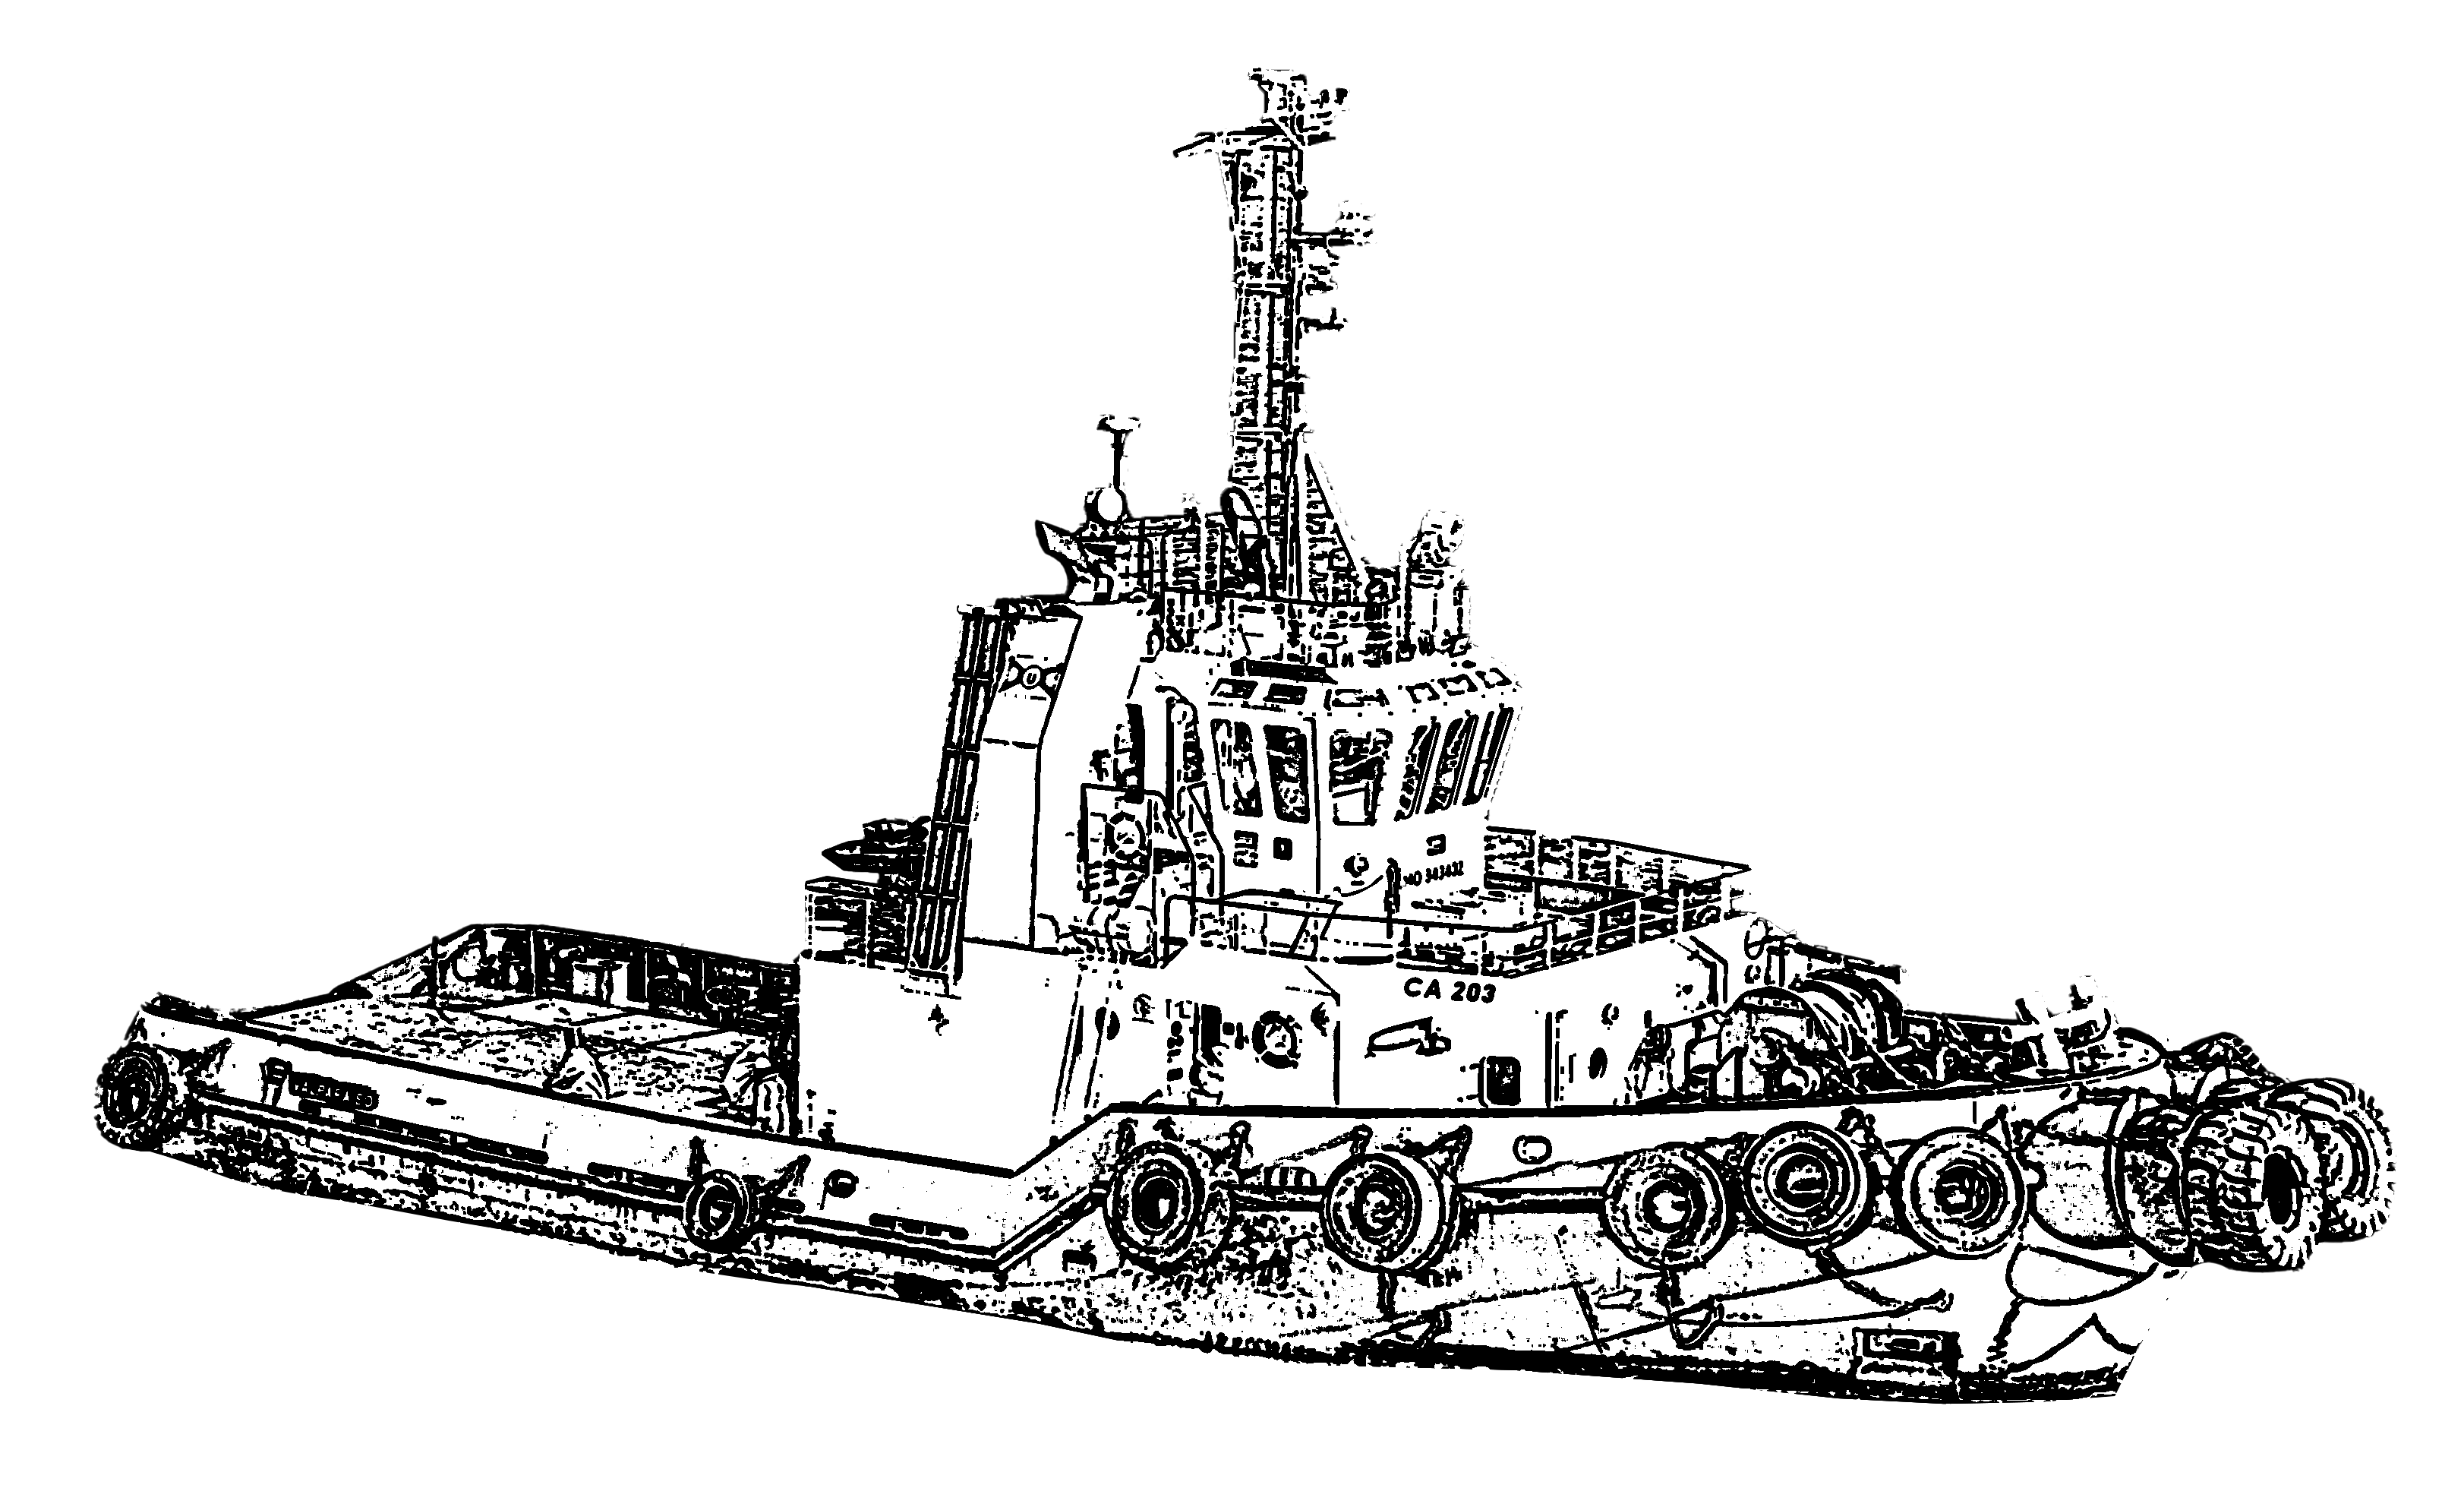
\includegraphics[width=1\textwidth]{images/chapter02/Remolcador.png}
    \caption{Conventional tug representation.}
    \label{fig:Tug1}
    \end{subfigure}
    \begin{subfigure}{0.5\textwidth}
    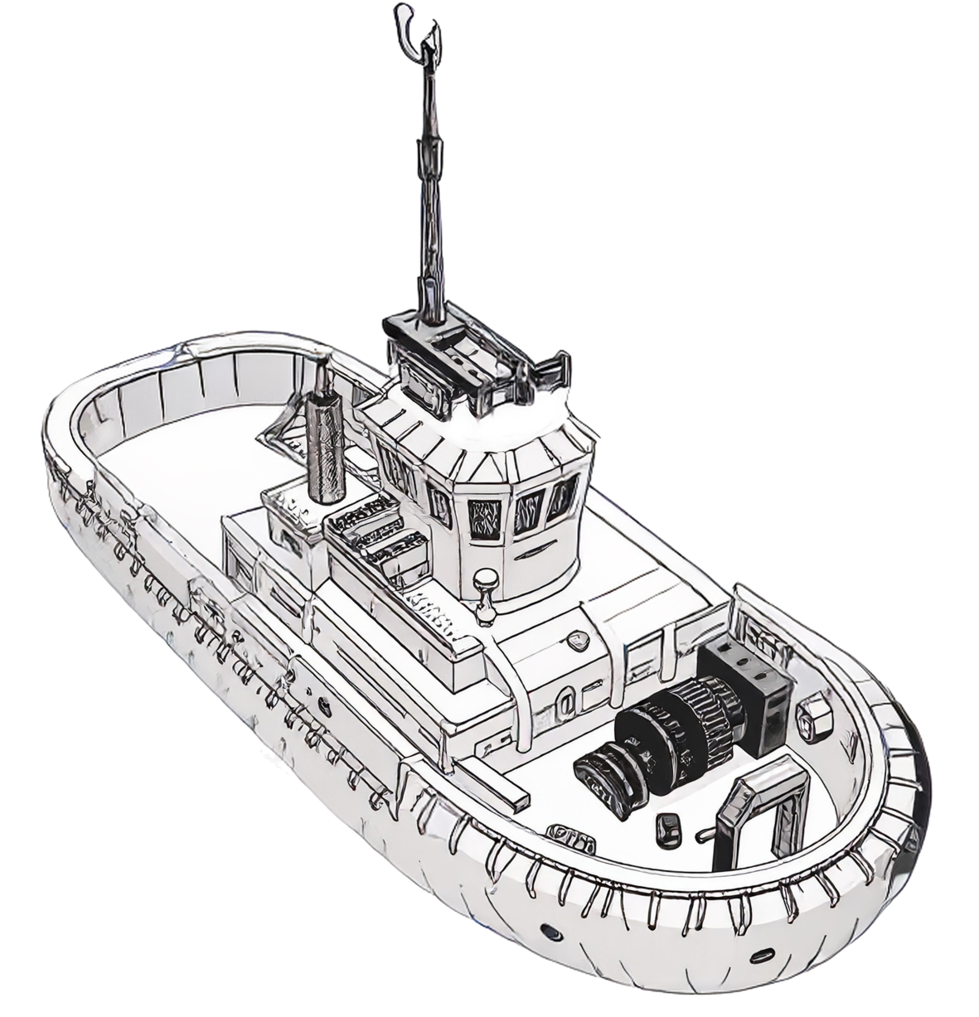
\includegraphics[width=0.7\textwidth]{images/chapter02/Remolcador2.png}
    \caption{Azimuth Tug representation}
    \label{fig:Tug2}
    \end{subfigure}    
    \caption{Tugs representations}
    \label{fig:Tugs}
\end{figure}

A tugboat is technically defined as a type of vessel specifically designed to assist other ships in moving by providing a controlled amount of force. They are essential vessels in ports, as is shown in fig. \ref{fig:Tugs}, where they assist in the movement of floating objects and in emergency tasks \cite{INEAL}.

In maritime law, maritime towing is defined as the operation whereby a vessel (the tugboat) transports another vessel or floating device that lacks self-propulsion or, despite having it, is unable to navigate under its own power, by pulling it through the sea. This functional duality—which encompasses both high-precision maneuvering assistance in congested environments (port towing) and long-distance transport and salvage (offshore towing)—requires design engineering and system redundancy adapted to very different operational risks \cite{Bruce}.

The importance of tugboats has grown exponentially with the phenomenon of naval gigantism \cite{Murimar}. Large modern ships, such as cruise ships and oil tankers, have tremendous momentum (inertia) that prevents them from stopping quickly or maneuvering effectively on their own in narrow channels or docks \cite{ESC_Group}.   

Therefore, tugboats are essential to counteract these inertial forces. Support is necessary for entry, exit, and general maneuvering, including assisting ships in emergency situations  \cite{Bruce}.   

Technological innovation plays a key role in tugboat operations. Environmental challenges and high efficiency requirements have driven the digitization and development of more sustainable and less polluting tugboats \cite{Murimar}. This trend includes the integration of automatic control technologies to optimize maneuver management, such as investment in hybrid and electric propulsion systems.\\\\     









The efficiency of these types of vessels is based on fuel consumption in relation to load capacities, always taking into account both the propulsion system and the energy conversion system that determines it. The efficiency of conventional propulsion systems varies between 38$\%$ and 41$\%$ for a power range between 100 kW and 2,500 kW. For vessels with higher power ratings, efficiency increases to 48$\%$ \cite{Griffiths} \cite{Wik}.

\subsection{Types of tugboats}
%(port, deep-sea, coastal, escort, etc.)
The classification of tugboats is primarily based on their operational domain and assigned primary mission. The usage and functions of tugs vary from port to port, as different ports have different requirements and intakes. The common thing is pushing or towing mega boats or barges. Their usage depends on the following factors:

\begin{itemize}
\item Port traffic Volume,
\item Types of ships to be served by that tug,
\item Navigational obstacles to be catered to,
\item Conditions of environmental protection,
\item Local laws and
\item Domains to be carried by a tug.
\end{itemize}

\subsubsection{a) Harbour Tugs}
These vessels are specialized in assisting large ships entering and leaving port limits. Their design prioritizes agility and the ability to apply force in any direction with maximum efficiency \cite{INEAL}. 

\begin{itemize}
	\item \textbf{Design:} Typical dimensions vary in length between 20 and 30 meters, with drafts of 3.0 to 4.5 meters. Their empty displacement speed ranges from 5 to 13 knots (9.3 - 24 km/h). The power of these tugboats can vary considerably, generally between 400 - 3,000 hp (300 and 2200 kW)\cite{IngeMarino}.
	
	
	\item \textbf{Propulsion:} Their designs have reduced length and increased beam and depth in order to install greater propulsion power, variable pitch propellers, Kort-type rotating nozzles with fixed rudders or rudder flaps, or Tow-Master systems (fixed nozzles with five rudders, two at the bow and three at the stern) to achieve greater traction and maneuverability \cite{IngeMarino} \cite{PracticosPuerto}.
\end{itemize}

\subsubsection{b) Offshore/SAR Tugs}
Designed to operate in the open sea, these tugboats are characterized by their robustness, greater autonomy, and ability to withstand severe ocean conditions.

\begin{itemize}
	 \item \textbf{Design:} Typical dimensions vary in length between 25 and 40 meters, with drafts of 4.5 to 6 meters. Their empty displacement speed ranges from 5 to 13 knots (9.3 - 24 km/h). The power of these tugboats can vary considerably, generally between 1500 - 6,000 hp (1120 - 4470 kW)\cite{IngeMarino}.

	\item \textbf{Multifunctionality:} In addition to long-distance towing tasks, they are equipped for rescues and complementary firefighting and pollution control tasks \cite{SalvamentoMaritimo}. An example of a modern rescue vessel is 40 meters long, has 5,300 hp and a Bollard Pull of 60 tons \cite{Cotecmar}. These vessels are equipped to provide any type of assistance to deep-draft vessels \cite{SalvamentoMaritimo}. 
\end{itemize}

\subsubsection{c) Escort Tugs}
These tugboats perform a critical safety mission. Their main objective is to provide preventive escort to ships carrying hazardous materials (such as LNG or crude oil) in high-risk areas, standing ready to counteract any possible loss of control of the assisted vessel.

\begin{itemize}

	\item \textbf{Design:} Typical dimensions vary in length between 40 and 80 meters, with drafts of 5 to 6 meters. Their empty displacement speed ranges from 15 to 16 knots (9.3 - 24 km/h). The power of these tugboats can vary considerably, generally between 6,000 -20,000 hp (4470 - 14,900 kW)\cite{IngeMarino}.

	\item \textbf{Technology and Bollard Pull:} They require extremely robust and powerful designs to maintain control of a vessel moving at cruising speeds. An example of a modern escort tugboat (\textit{Robert Allan Rastar 3200 model}) features Rolls Royce azimuth thrusters and is designed to generate fixed-point traction exceeding 85 tons \cite{PortalPortuario}. They are equipped with constant tension maneuvering winches to maximize safety during operations. 
\end{itemize}


\subsubsection{d) Tugs Comparation}

Below, in the table \ref{tab:Tugs}, there is a summary of key operational and dimensional characteristics:

\begin{table}[H]
	\centering
	\caption{Operational Classification and Dimensional Parameters of the Tugboat}
	\label{tab:Tugs}
	\begin{tabular}{c|p{35mm}|p{35mm}|c}
		\hline      \textbf{Type of Tugboat} & \textbf{Operation}  & \textbf{Design objective} & \textbf{Typical BP} \\		
\hline \hline
		Harbour Tug    & Protected maritime and port areas such as bays or estuaries. & Maneuverability, Reduced Draft & 40-80\\ \hline
		Offshore/SAR Tugs  & Open Ocean & Autonomy, Stability, SAR Power & 60-200+\\ \hline
		Escort Tugs  & High-Risk Areas (LNG, Crude Oil) & Rollover Control, Side Pull Capacity & 60-120\\
		\hline \hline
	\end{tabular}
\end{table}



\section{Technical Characteristics of the Propulsion System}

% Explicar las características mecánicas y eléctricas que determinan cómo debe diseñarse el sistema híbrido.

\subsection{Bollard Pull - BP}
Bollard pull (BP) is the fundamental metric for quantifying a tugboat's pulling power.

BP measures the maximum force a vessel can exert while stationary in the water. It is the maritime equivalent of horsepower or torque in land vehicles. The measurement requires securing the vessel to a fixed bollard at the dock and using specialized load cells to calculate the tension generated on the line with the engines running at full power.   

BP specifications are expressed in units such as kilonewtons (kN), short tons (stf), or ton-force (tf) and are critical for demonstrating the vessel's pulling capacity under load. All commercial vessels intended for towing operations must obtain fixed point pulling certification from international classification societies such as the American Bureau of Shipping (ABS) or Bureau Veritas (BV)\cite{Murimar}.   

The tugboat's design is specifically geared toward maximizing pulling force in relation to its size. A common and effective way to increase pulling force is by adding a nozzle (duct) that surrounds the propeller, which improves propulsive efficiency \cite{Murimar}. 

\subsection{Propulsion Engineering for Maneuvering}
The maneuverability of a tugboat, which directly influences its operational efficiency and safety, is intrinsically linked to the design of its propulsion system.

\subsubsection{a) Conventional Propulsion} It uses a standard diesel engine connected to a propeller. It is a proven and simple system, with good efficiency in linear towing tasks within ports and coastal areas. However, it offers limited lateral maneuverability compared to more advanced systems \cite{MJimenez}.

\subsubsection{b) ASD - Azimuthal Stern Drive} These are rotary thrusters, where a motor is capable of directing all its thrust in any direction \cite{MJimenez}. They all have two propellers, and since each one can be oriented independently, maneuverability is greatly increased, allowing them to turn on themselves in a single length \cite{JFarina}. The only difference with conventional tugboats are the modifications to the stern and structure to house the propellers and withstand the forces exerted by the nozzle rudder, which are different from those exerted by a conventional rudder and propeller \cite{JFarina}. 

\subsubsection{c) Voith-Schneider Propulsion (VSP)} This system offers omnidirectional thrust and total steering control, resulting in formidable positioning accuracy. These harbor tugs have been equipped with \textit{VoithSchneider} propellers, a unique type of propulsion system consisting of oscillating blades that allow them to have total, targeted control over the vessel without having to adjust the orientation of the main engine or propellers \cite{MJimenez}.

This propulsion system allows for highly precise operation in any direction due to its agility, making it ideal for rescue operations as well as in ports crowded with high-density maritime traffic \cite{MJimenez}.

\subsubsection{d) Propulsion Comparation }

\begin{table}[H]
	\centering
	\caption{Comparison of Propulsion Systems in Tugboats and Performance.}
	\label{tab:Prop_Comp}
	\begin{tabular}{c|p{35mm}|p{35mm}|p{35mm}}
		\hline      \textbf{Propulsion System} & \textbf{Advantages}  & \textbf{Maneuverability} & \textbf{Typical Application} \\		
\hline \hline
		Conventional    & Low Cost, Proven Design & Limited (Good in a straight line) & Single Coastal/Offshore Trailer\\ \hline
		ASD  & High BP, Axis Rotation, Port Agility & Good & Port Towing and Escort\\ \hline
		VSP  & Omnidirectional Thrust, Extreme Stability & Very Good & Congested Ports \\
		\hline \hline
	\end{tabular}
\end{table}

\section{Propellers}

\section{Naval Maneuvers and Assistance Techniques}

Towing operations are governed by strict procedures that seek to maximize safety in dynamic and often restricted environments.	

\subsection{Docking and Undocking Procedures}

The assistance of tugboats is crucial during docking and undocking maneuvers. The undocking maneuver can be as laborious as the docking maneuver and must be planned in advance. The objective is to leave the assisted vessel clear of the dock, in a safe position that allows the rudder and propeller to be effective so that the vessel can gain control and momentum.

\subsubsection{a) Operational Coordination}

The maneuver is initiated by request via VHF radio. The bow and stern operating personnel receive instructions to unmoor the lines.

\subsubsection{b) External Agent Management}
It is essential to consider the effects of winds and currents. Strong winds from outside can add to the effects of the engine in reverse during undocking, creating a dangerous situation that can violently push the stern or bow toward the dock. The ability of the highly maneuverable tugboat to apply instantaneous lateral force reduces the time the assisted vessel is exposed to the combined and unfavorable action of wind and propulsion, mitigating the risk of collision. If the wind action is severe, tugboat assistance is mandatory, especially if the actions of the assisted vessel's capstan are insufficient.

\subsection{Tugboat Performance}
Tugboats use various configurations to apply controlled force:

\subsubsection{a) Tugboat Working on a Beam or Over a Cable}
The tugboat tows or holds the assisted vessel via a remote towline. This is the typical form of towing in transit.

\subsubsection{b) Bow-Supported Tugboat (Ram Locking)}
The tugboat applies direct thrust force against the side of the assisted vessel, using its fenders, often to rotate or move the vessel sideways.

\subsubsection{c) Tugboat alongside}
The tugboat is securely moored alongside the larger vessel. This technique provides very precise lateral and rotational control, which is essential for maneuvering wide-beam vessels in narrow channels. 


\section{Operational Profile}
%Aquí se describe cómo opera el remolcador durante un día típico o misión.
Next, we will analyze the operating profile of a tugboat in Chile, considering that it has an operating schedule of 10 working hours, performing this work in Puerto Montt.

\subsection{Brake-Specific Fuel Consumption (BSFC)}

\begin{figure}[H]
    \centering
    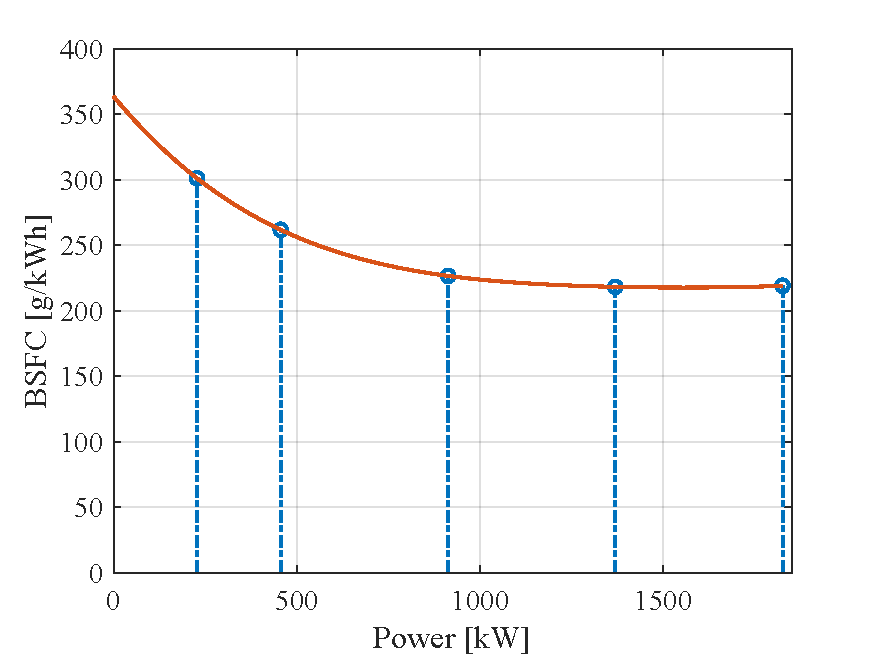
\includegraphics[scale=1]{images/chapter02/BSFC.pdf}
    \caption{Brake-specific fuel consumption (BSFC) of the \textit{CAT 3516B engine} used in tugboats.}
    \label{fig:BSFC}
\end{figure}

To analyze the operating profile, it is necessary to introduce the concept of \textbf{brake-specific fuel consumption (BSFC)}. BSFC is a measure of an engine's fuel efficiency, calculated as the amount of fuel consumed per unit of power produced over a specific time \cite{LSZ}. 

The BSFC as a function of output power is illustrated in fig. \ref{fig:BSFC} for a typical engine used in tugboats. At higher power levels, the BSFC is lower, indicating that more power is produced per unit of fuel, resulting in greater efficiency. Maximum efficiency is achieved at the engine's rated power, where it operates as intended, maintaining an optimal balance between fuel consumption and power output. Conversely, at lower power levels, the BSFC is higher, meaning that fuel consumption per unit of power is greater, thus reducing the engine efficiency.

The relative efficiency evaluates how the conventional engine is working taking as a reference the optimal efficiency at the nominal operating point as shown in eq. \ref{eq:rel_eff}. At this operating point the relative efficiency is 100$\%$ reducing its value if the engine works at lower levels of power.

\begin{align}\label{eq:rel_eff}
    \eta_\text{rel} &= \frac{\text{BSFC}_\text{nom}}{\text{BSFC}}
\end{align}

\subsection{Generated Emissions and Fuel Consumption}

To calculate emissions, the following formula relates brake power (Pb), BSFC, usage time (tu), and a carbon factor (CF):

\begin{align}
    \text{Emissions} &= \frac{\text{BSFC} \cdot {P}_{b} \cdot {t}_{u} \cdot \text{CF}}{10^{-6}} \quad \text{[t CO\textsubscript{2}]}
\end{align}

\begin{figure}[!t]
    \centering
    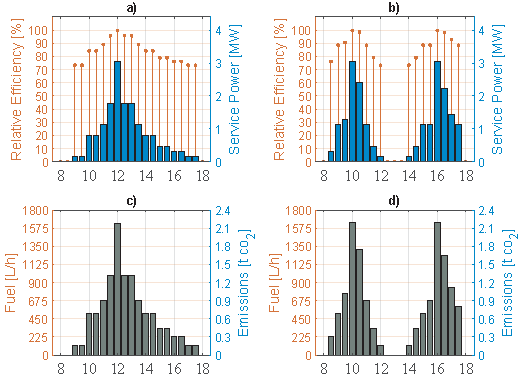
\includegraphics[width=1\linewidth]{images/chapter02/pot_30min.pdf}
    \caption{Load profile of a tugboat operating in a Chilean harbor: a) One service manoeuvre, b) Two service manoeuvres, c) Fuel consumption/emissions generated for a service maneuver, d) Fuel consumption/emissions generated for two service maneuvers.}
    \label{fig:load profile}
\end{figure}

The operational profile of a tugboat operating in a Chilean port typically includes one to two maneuvers per day during a 10-hour work shift, as illustrated in Fig. \ref{fig:load profile}.
Fig. \ref{fig:load profile}-a) shows the power delivered by the tugboat conventional propulsion system and the relative efficiency of the engines during one service maneuver while b) shows the same information for two maneuvers; c) shows the fuel consumption by the tug and the CO\textsubscript{2} emissions generated by the load of the diesel engines, corresponding to a maneuver, while d) shows the emissions generated by the load of the diesel engines for two service maneuvers.

\begin{figure}[H]
    \centering
    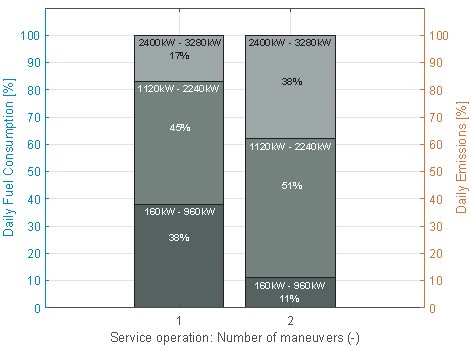
\includegraphics[width=0.9\linewidth]{images/chapter02/operations.pdf}
    \caption{Percentage of emissions per day based on power ranges.}
    \label{fig:emmis}
\end{figure}


It can be observed that as the tugboat operates close to the nominal power point of its diesel engines, its relative efficiency improves. This indicates optimal fuel consumption during those periods. Conversely, at lower operating points, the engine consumes more fuel relative to the energy produced.



Fig. \ref{fig:emmis} shows the accumulated fuel consumption and CO\textsubscript{2} emissions generated for one and two maneuvers. Each service operation is divided into three segments: the lower segments correspond to propulsion system power levels with a relative efficiency below 90\%, the middle segments correspond to relative efficiencies ranging from 90\% to 98\%, and the upper segments represent power levels with the highest relative efficiency, ranging from 98\% to 99.8\%.  At low power levels, fuel consumption can account for up to 38\% and 11\% of the total daily fuel usage, for one and two maneuvers, respectively. Resulting in high emissions due to the diesel engine operating far from its optimal efficiency point, emphasizing the variability of the load profile of this type of vessel and its impact on fuel consumption and emissions. 
 
\section{Chapter Summary}
    \chapter{Hybrid Tugboats: Requirements and Performance}

This chapter presents the fundamental concepts associated with tugboat hybridization, its most common technological configurations, and the operational benefits associated with the incorporation of battery banks. The objective is to establish the theoretical and technical basis for the design process carried out in subsequent chapters.

\section{General concepts of marine hybrid systems}
Given the intermittent nature of the load profile and the dependence on diesel engines, which are oversized for low-load tasks, the implementation of the hybrid energy storage system proposed in this thesis is analyzed.

The first step is to take a closer look at the existing types of hybridization:

\section{Classification of Hybrid Propulsion Systems}

The maritime industry has evolved distinct topological approaches to hybridization, each offering specific trade-offs between complexity, cost, redundancy, and efficiency.

\subsection{Series Hybrid Architecture}

In a series hybrid configuration, the mechanical link between the internal combustion engine and the propeller shaft is severed completely. The vessel is propelled exclusively by electric motors.

The main diesel engines function strictly as generator sets (gensets). They produce electrical energy which is rectified (if AC) and fed into a common distribution bus. This bus supplies power to variable frequency drives (VFDs) that control the electric propulsion motors. The decoupling of engine speed from propeller speed is the primary advantage here. A fixed-pitch propeller’s torque curve is cubic; at low speeds, it requires very little torque. A diesel engine, however, cannot run stable below a certain RPM (typically 600-800 RPM). In a series hybrid, the genset can run at its optimal constant RPM (e.g., 1500 or 1800 RPM) to generate the exact amount of current needed by the motor, or it can shut down while the battery takes over.

\begin{itemize}
	\item \textbf{Electric Shaft}:  Here, power is transformed by electric machines without intermediate power electronics for the main transmission path, although this is rarer in modern DC-based designs.
	\item \textbf{DC Link Topology}: This is the modern standard. Mechanical power is converted to electricity, fed into a DC bus (often 1000V DC), and then inverted back to AC for the propulsion motors. This topology allows for independent control of multiple propulsors without variable pitch mechanisms and integrates energy storage seamlessly
\end{itemize}

Series hybrids are ideal for "stop-and-go" vessels like city ferries or tugs that operate predominantly at low speeds. The battery bank in a series hybrid is often larger to buffer the high power demands of the electric motors. However, at full continuous speed, series hybrids suffer from "round-trip efficiency losses." converting mechanical energy to electrical and back to mechanical incurs a penalty of approximately 5-10$\%$ compared to a direct mechanical shaft.

\subsection{Parallel Hybrid Architecture}

\begin{itemize}
	\item Configuración Técnica
	\item Variaciones
	\item Escenarios
	\item Ejemplo de embarcación
\end{itemize}

In this setup, both the internal combustion engine and an electric machine (motor/generator) are mechanically connected to the propeller shaft, typically via a reduction gearbox with complex clutching arrangements. The electric machine is usually mounted as a PTI (Power Take-In) / PTO (Power Take-Out) unit.

\begin{itemize}
	\item \textbf{Mechanical Mode}: The main diesel engine drives the propeller directly. This is used for heavy towing and high-speed transit. The electric machine may freewheel or act as a generator (PTO) to charge batteries.
	\item \textbf{Electric Mode (Green Mode)}: The main diesel engine is declutched and shut down. The electric motor, powered by the battery or an auxiliary genset, drives the shaft. This is used for loitering (0-6 knots) and "silent" harbor transit.
	\item \textbf{Boost Mode}: Both the diesel engine and the electric motor provide torque to the shaft simultaneously. This allows the vessel to achieve a total power output greater than the rating of the main engine alone, providing the "peak" power needed for emergency ship assist maneuvers without requiring a larger main engine.   


\end{itemize}

\subsection{Comparation}

The parallel hybrid architecture is currently the dominant configuration for high-bollard-pull tugs because it preserves the mechanical efficiency of the direct drive for peak loads.


\section{Power Generation and Energy Storage System}

The hybrid tugboat relies on a triad of power sources: Main Propulsion Engines, Auxiliary Generators, and the Battery Energy Storage System (BESS). The roles of these components have shifted significantly from conventional designs.

\subsection{Main Propulsion Diesel Engines}

Because the electric motor handles low-speed maneuvering and idling, the main engines are only started when high power is actually needed. This dramatically reduces their running hours—often by 50$\%$ or more—extending the time between overhauls (TBO).

The mechanical connection allows the engine to deliver its full rated power to the shaft, supplemented by the electric motor. This allows designers to install slightly smaller main engines (saving weight and cost) while still meeting maximum bollard pull requirements via the battery boost.

\subsection{Auxiliary Diesel Generators}

In a conventional tug, auxiliary generators (gensets) power the lights and galley. In a hybrid tug, they are critical propulsion components. 

They are the primary source of energy, often arranged in banks (e.g., 4 x smaller gensets instead of 2 x large main engines). This allows for granular power management—running only 1 genset for low speed, and 4 for full speed.

They act as range extenders. If the battery is depleted during "Green Mode," the auxiliary genset starts up to power the electric motor (PTI) and recharge the battery, avoiding the startup of the large main engines for low-power tasks.   

\subsection{Battery Bank}

The BESS is the heart of the hybrid system. Its role extends far beyond simple energy storage; it is a dynamic stability tool that fundamentally alters how the diesel engines are operated.

\subsubsection{a) Peak Shaving}

Tugboats experience extreme load transients. When a tug engages a tow line, the load on the propeller can jump from 0$\%$ to 100$\%$ in seconds. A diesel engine struggles to handle this ramp-up rate without thermal stress and incomplete combustion (black smoke). The BESS acts as a capacitor, discharging instantly to meet this spike. This allows the diesel engine to ramp up slowly along its optimal thermal curve. Mechanism: The Energy Management System (EMS) detects a load step. It commands the DC/DC converters on the battery to discharge, supplying the immediate torque demand to the motor. As the diesel engine slowly increases RPM, the battery contribution tapers off. 

\subsubsection{b) Spinning Reverse}

Regulatory bodies and safety guidelines (such as those from DNV and ABS) typically require redundancy during critical maneuvers. Conventionally, this means running a second standby engine even if the load doesn't require it. Mechanism: The BESS serves as a "virtual generator." If the active diesel generator fails, the battery instantaneously picks up the load, preventing a blackout. This capability, recognized by DNV's Battery(Power) notation, allows the operator to keep the standby engine off, saving fuel and engine hours.

\subsubsection{c) Load Levelling (Optimization)}
Diesel engines are most efficient at high loads (approx. 85$\%$). Mechanism: If the propulsive demand is only 50$\%$, the EMS runs the engine at 85$\%$ load. The excess 35$\%$ is diverted to charge the batteries. Conversely, if the load is 110$\%$, the engine remains at its MCR (100$\%$), and the battery supplies the extra 10$\%$ (Boost Mode). This ensures the engine never operates in the inefficient "wet stacking" zone.
 

\section{Grid Distribution}

Traditional ships use 440V or 690V AC grids, but the integration of batteries (DC sources) and variable speed drives (DC internal) makes AC inefficient and cumbersome.
The architectural shift from Alternating Current (AC) to Direct Current (DC) distribution is the technological enabler of modern hybrid vessels.

\subsection{DC Link}

The industry standard for modern hybrid tugs has coalesced around the 1000V DC grid. This voltage level allows for power distribution up to approximately 20MW, which covers the requirements of even the largest offshore support vessels and tugs.

Distributing power at 1000V DC rather than 690V AC reduces current for the same power transfer, allowing for smaller cable cross-sections. Furthermore, DC does not suffer from the "skin effect" or reactive power losses, allowing for a reduction in cabling mass of up to 40$\%$.

In an AC grid, generators must run at a fixed speed (e.g., 1800 rpm for 60Hz) to maintain frequency, regardless of load. In a DC grid, the engine speed can be decoupled from the grid frequency. The engine can slow down to idle speeds during low load while still producing the required voltage, resulting in fuel savings of up to 20$\%$.

The Onboard DC Grid concept eliminates the need for bulky propulsion transformers and main AC switchboards. This can reduce the total footprint of the electrical equipment by 30$\%$ to 75$\%$, freeing up valuable space in the cramped machinery spaces of a tugboat.

\subsection{AC Link}

FALTA INFO

\subsection{Comparation}

Comparative studies highlight the superiority of DC links in hybrid applications.

\begin{itemize}
	\item \textbf{Conversion Losses}: n a traditional drive with an AC grid, power flows: Generator (AC) $\to$ Switchboard (AC) $\to$ Rectifier (DC) $\to$ Inverter (AC) $\to$ Motor. With a DC grid, the "Rectifier" stage is centralized or integrated, and batteries connect directly to the DC bus via DC/DC converters. This eliminates multiple conversion steps.
	\item \textbf{System Efficiency}: Studies indicate a system-level efficiency improvement of 0.5–1$\%$ for DC grids over AC grids purely on conduction losses, but the operational efficiency gains (due to variable speed engines and battery integration) often exceed 20$\%$.
\end{itemize}


\section{Service Maneuvers of a Hybrid Tugboat}

\subsection{Operational Profile}

\subsection{Generated Emissions and Fuel Consumption}
	
\subsection{Chapter summary}
    \chapter{Preliminary design of the battery bank for a hybrid propulsion system}

This chapter presents the preliminary design process for the battery bank required for the tugboat's hybrid propulsion system. The energy capacity, power requirements, and operating constraints are determined, and then different storage technologies are evaluated from a technical and economic perspective.

\section{Design parameters and initial assumptions}

\subsection{Operational assumptions}

\subsection{Energy design parameters}

\subsection{Power design parameters}

\subsection{Physical and regulatory constraints}

\section{Battery bank sizing}

\subsection{Calculation of required energy capacity (kWh)}

\subsection{Calculation of required power (kW)}

\section{Battery technologies applicable to tugboats}

\subsection{Selection criteria}

\subsection{Technology analysis}

\section{Economic and life cycle analysis}

\subsection{System CAPEX}

\subsection{System OPEX}

\subsection{ROI / VAN / TIR / Payback}

\section{Comprehensive comparison of alternatives}

\subsection{Selection of the optimal alternative}

\section{Chapter Summary}
    \input{content/chapter05}
    \chapter{Conclusions}

The development of a hybrid propulsion system through retrofitting involves multiple variables, with the technical and economic analysis of the battery bank as the central focus. The characterization of the load profile is the starting point, allowing the inefficiencies of the original system to be quantified and a battery bank to be sized according to the ship's operational requirements.\\
In addition to the technical analysis of the battery bank, it is crucial to integrate regulatory frameworks and physical limits (weight and volume), which are determining factors in the architecture of a tugboat. At the same time, profitability analysis—considering the optimal level of hybridization according to the asset's useful life—is vital to ensure return on investment (ROI) and attract capital interested in maritime decarbonization.\\

Once the technical and economic feasibility has been validated, mathematical modeling and subsequent analysis of the electrical performance of the battery bank and power converters are carried out. This comprehensive approach not only ensures that the system meets the demands of the propulsion system, but also establishes a robust methodology with multiple criteria, seeking to ensure that hybridization processes are successful and aligned with global emissions policies. In this way, this work seeks to lay the foundations for the creation of a methodology that allows the modeling of battery banks for hybrid tugboats, considering multiple variables in the design process.


    \chapter*{Future Work}

Based on the methodology presented in this paper, it is proposed as future work:

\begin{itemize}
	\item Model the other internal elements of the hybrid powertrain to ultimately obtain a simulated model of the propulsion system that allows different load profiles to be tested.
	\item Based on the information provided in this paper, related to technical and economic aspects, the aim is to work on an optimization function that incorporates information from all these areas and allows us to identify the best battery alternatives, optimizing variables such as project cost, number of cells, available space, etc.
	\item The complexity of the battery bank model can be increased by adding dynamics that provide a better understanding of performance when a more detailed load profile is obtained, not only in terms of hours but also in terms of minutes or seconds.
	\item Implement PTO mode and analyze the feasibility of replacing diesel engines with ones with lower nominal power, allowing the use of batteries for towing tasks.
	\item Consideration of port charger implementation, which could also impact the economic analysis of hybridization.
	\item Through sensorization, monitor the health status of the different elements within the hybrid power system, especially the battery bank, in order to generate predictive maintenance routines and also have an operating history.
\end{itemize}
    \appendix
    \chapter{Appendix}



\section{CO\textsubscript{2} tax emissions}\label{sec:tax}

In countries such as Finland, there is a so-called carbon tax, which seeks to mitigate the effects of climate change by discouraging the use of fossil fuels 
\cite{UnitedNAtions}.

Based on this, a carbon tax of $ \$50/{\text{ton}}_{\text{CO\textsubscript{2}}}$ will be assumed, and the impact this has on economic sensitivity variables will be determined,  since this tax mainly affects the OPEX related to each battery.

\subsection{Net Present Value (NPV)}

\begin{table}[H]
	\centering
	\caption{Calculated NPV, with carbon taxes, without  subsides (small bank).}
	\label{tab:van1c}
	\begin{tabular}{|c|c|c|c|}
		\hline
		\multicolumn{4}{|c|}{Battery Bank $15\%$ ${\text{P}}_{\text{nom}}$} \\
		\hline\hline
	Lifespan  & 10 years & 15 years & 20 years\\
		 \hline
    ${\text{NPV}}_{\text{NMC}}$ & $\$241,940$ & $\$1,545,943$ & $\$2,433,426$\\
		 \hline
	${\text{NPV}}_{\text{LFP}}$ & $\$1,929,657$ & $\$3,354,487$ & $\$4,324,203$\\
		 \hline
 	${\text{NPV}}_{\text{LTO}}$ & $\$1,007,204$ & $\$2,587,384$ & $\$3,662,827$\\
		 \hline
	\end{tabular}
\end{table}

\begin{table}[H]
	\centering
	\caption{Calculated NPV, with carbon taxes and without subsides (large bank).}
	\label{tab:van2c}
	\begin{tabular}{|c|c|c|c|}
		\hline
		\multicolumn{4}{|c|}{Battery Bank $25\%$ ${\text{P}}_{\text{nom}}$} \\
		\hline\hline
	Lifespan  & 10 years & 15 years & 20 years\\
		 \hline
    ${\text{NPV}}_{\text{NMC}}$ & -$\$3,340,207$ & $-\$2,156,302$ &-$\$1,350,557$\\
		 \hline
	${\text{NPV}}_{\text{LFP}}$ & -$\$71,650$ & $\$1,384,116$ & $\$2,374,886$\\
		 \hline
 	${\text{NPV}}_{\text{LTO}}$ & -$\$1,792,895$ & $\$176,901$ & $\$1,517,511$\\
		 \hline
	\end{tabular}
\end{table}

\subsection{Internal Rate of Return (IRR)}

\begin{table}[H]
	\centering
	\caption{Calculated IRR, with carbon taxes and without subsides (small bank).}
	\label{tab:tir1c}
	\begin{tabular}{|c|c|c|c|}
		\hline
		\multicolumn{4}{|c|}{Battery Bank $15\%$ ${\text{P}}_{\text{nom}}$} \\
		\hline\hline
	Lifespan  & 10 years & 15 years & 20 years\\
		 \hline
    ${\text{IRR}}_{\text{NMC}}$ & $9.18\%$ & $13.29\%$ & $14.69\%$ \\
		 \hline
	${\text{IRR}}_{\text{LFP}}$ & $19.91\%$ & $22.67\%$ & $23.43\%$\\
		 \hline
 	${\text{IRR}}_{\text{LTO}}$ & $12.52\%$ & $16.17\%$ & $17.34\%$\\
		 \hline
	\end{tabular}
\end{table}

\begin{table}[H]
	\centering
	\caption{Calculated IRR, with carbon tax and without subsides (large bank).}
	\label{tab:tir2c}
	\begin{tabular}{|c|c|c|c|}
		\hline
		\multicolumn{4}{|c|}{Battery Bank $25\%$ ${\text{P}}_{\text{nom}}$} \\
		\hline\hline
	Lifespan  & 10 years & 15 years & 20 years\\
		 \hline
    ${\text{IRR}}_{\text{NMC}}$ & $-3.08\%$ & $3.01\%$ & $5.52\%$ \\
		 \hline
	${\text{IRR}}_{\text{LFP}}$ & $7.70\%$ & $12.03\%$ & $13.54\%$\\
		 \hline
 	${\text{IRR}}_{\text{LTO}}$ & $1.63\%$ & $6.91\%$ & $8.95\%$\\
		 \hline
	\end{tabular}
\end{table}

\subsection{Return on Investment (ROI)/ Payback Period}

\begin{table}[H]
	\centering
	\caption{Calculated period for positive ROI, with carbon taxes and without subsides (small bank).}
	\label{tab:roi1c}
	\begin{tabular}{|c|c|}
		\hline
		\multicolumn{2}{|c|}{Battery Bank $15\%$ ${\text{P}}_{\text{nom}}$} \\
		\hline\hline
		    & \textbf{Period}\\
		 \hline
	${\text{ROI}}_{\text{NMC}}>0$ & $\approx$ 6 years and 5 months\\
		 \hline
	${\text{ROI}}_{\text{LFP}}>0$ & $\approx$ 4 years and 3 months\\
		 \hline
 	${\text{ROI}}_{\text{LTO}}>0$ & $\approx$ 5 years and 7 months\\
		 \hline
	\end{tabular}
\end{table}

\begin{table}[H]
	\centering
	\caption{Calculated period for positive ROI, witho carbon taxes and without subsides (large bank).}
	\label{tab:roi2c}
	\begin{tabular}{|c|c|}
		\hline
		\multicolumn{2}{|c|}{Battery Bank $25\%$ ${\text{P}}_{\text{nom}}$} \\
		\hline\hline
		    & \textbf{Period}\\
		 \hline
	${\text{ROI}}_{\text{NMC}}>0$ & $\approx$ 11 years and 7 months \\
		 \hline
	${\text{ROI}}_{\text{LFP}}>0$ & $\approx$ 6 years and 7 months \\
		 \hline
 	${\text{ROI}}_{\text{LTO}}>0$ & $\approx$ 8 years and 11 months\\
		 \hline
	\end{tabular}
\end{table}

\section{Government grants}\label{sec:grant}
With the aim of contributing to carbon neutrality in the global maritime transport sector, there are government programs that promote the use of clean technologies that accelerate decarbonization, such as the Ministry of Oceans and Fisheries of the Republic of Korea (MOF), which announced its "First National Plan for the Development and Popularization of Eco-friendly Ships (2021-2030),“ known as the ”2030-K Eco-friendly Ship Promotion Strategy" \cite{mof}.

This strategy explores advanced zero-emission technologies that can reduce greenhouse gas (GHG) emissions in areas such as ship design, future fuels, renewable energy, and equipment, among others. In this way, the Ministry of Finance is facilitating the conversion of $15\%$ of Korean-flagged ships (528 out of a total of 3,542), for both the public and private sectors.\\

This will be considered a $10\%$ government subsidy, which will directly affect the CAPEX of each design and the economic sensitivity variables.

\subsection{Net Present Value (NPV)}

\begin{table}[H]
	\centering
	\caption{Calculated NPV, without taxes and with government grants (small bank).}
	\label{tab:van1s}
	\begin{tabular}{|c|c|c|c|}
		\hline
		\multicolumn{4}{|c|}{Battery Bank $15\%$ ${\text{P}}_{\text{nom}}$} \\
		\hline\hline
	Lifespan  & 10 years & 15 years & 20 years\\
		 \hline
    ${\text{NPV}}_{\text{NMC}}$ & -$\$150,908$ & $\$925,272$ & $\$1,657,703$\\
		 \hline
	${\text{NPV}}_{\text{LFP}}$ & $\$1,438,809$ & $\$2,635,817$ & $\$3,405,480$\\
		 \hline
 	${\text{NPV}}_{\text{LTO}}$ & $\$670,356$ & $\$2,022,713$ & $\$2,943,104$\\
		 \hline
	\end{tabular}
\end{table}

\begin{table}[H]
	\centering
	\caption{Calculated NPV, without taxes and with government grants (large bank).}
	\label{tab:van2c}
	\begin{tabular}{|c|c|c|c|}
		\hline
		\multicolumn{4}{|c|}{Battery Bank $25\%$ ${\text{P}}_{\text{nom}}$} \\
		\hline\hline
	Lifespan  & 10 years & 15 years & 20 years\\
		 \hline
    ${\text{NPV}}_{\text{NMC}}$ & -$\$3,545,391$ & $-\$2,261,373$ &-$\$1,992,502$\\
		 \hline
	${\text{NPV}}_{\text{LFP}}$ & -$\$497,334$ & $\$698,545$ & $\$1,512,441$\\
		 \hline
 	${\text{NPV}}_{\text{LTO}}$ & -$\$1,902,694$ & -$\$201,222$ & $\$956,771$\\
		 \hline
	\end{tabular}
\end{table}

\subsection{Internal Rate of Return (IRR)}

\begin{table}[H]
	\centering
	\caption{Calculated IRR, without taxes and with Government grants (small bank).}
	\label{tab:tir1s}
	\begin{tabular}{|c|c|c|c|}
		\hline
		\multicolumn{4}{|c|}{Battery Bank $15\%$ ${\text{P}}_{\text{nom}}$} \\
		\hline\hline
	Lifespan  & 10 years & 15 years & 20 years\\
		 \hline
    ${\text{IRR}}_{\text{NMC}}$ & $7.17\%$ & $11.57\%$ & $13.13\%$ \\
		 \hline
	${\text{IRR}}_{\text{LFP}}$ & $18.04\%$ & $21.01\%$ & $21.86\%$\\
		 \hline
 	${\text{IRR}}_{\text{LTO}}$ & $11.39\%$ & $15.16\%$ & $16.44\%$\\
		 \hline
	\end{tabular}
\end{table}

\begin{table}[H]
	\centering
	\caption{Calculated IRR, without taxes and with Government grants (large bank).}
	\label{tab:tir2c}
	\begin{tabular}{|c|c|c|c|}
		\hline
		\multicolumn{4}{|c|}{Battery Bank $25\%$ ${\text{P}}_{\text{nom}}$} \\
		\hline\hline
	Lifespan  & 10 years & 15 years & 20 years\\
		 \hline
    ${\text{IRR}}_{\text{NMC}}$ & $-5.47\%$ & $1.06\%$ & $3.82\%$ \\
		 \hline
	${\text{IRR}}_{\text{LFP}}$ & $5.66\%$ & $10.30\%$ & $11.98\%$\\
		 \hline
 	${\text{IRR}}_{\text{LTO}}$ & $0.63\%$ & $6.08\%$ & $8.21\%$\\
		 \hline
	\end{tabular}
\end{table}

\subsection{Return on Investment (ROI)/ Payback Period}

\begin{table}[H]
	\centering
	\caption{Calculated period for positive ROI, without carbon taxes and with government grants (small bank).}
	\label{tab:roi1s}
	\begin{tabular}{|c|c|}
		\hline
		\multicolumn{2}{|c|}{Battery Bank $15\%$ ${\text{P}}_{\text{nom}}$} \\
		\hline\hline
		    & \textbf{Period}\\
		 \hline
	${\text{ROI}}_{\text{NMC}}>0$ & $\approx$ 7 years\\
		 \hline
	${\text{ROI}}_{\text{LFP}}>0$ & $\approx$ 4 years and 6 months\\
		 \hline
 	${\text{ROI}}_{\text{LTO}}>0$ & $\approx$ 5 years and 10 months\\
		 \hline
	\end{tabular}
\end{table}

\begin{table}[H]
	\centering
	\caption{Calculated period for positive ROI, without taxes and with Government grants (large bank).}
	\label{tab:roi2c}
	\begin{tabular}{|c|c|}
		\hline
		\multicolumn{2}{|c|}{Battery Bank $25\%$ ${\text{P}}_{\text{nom}}$} \\
		\hline\hline
		    & \textbf{Period}\\
		 \hline
	${\text{ROI}}_{\text{NMC}}>0$ & $\approx$ 14 years and 9 months \\
		 \hline
	${\text{ROI}}_{\text{LFP}}>0$ & $\approx$ 8 years \\
		 \hline
 	${\text{ROI}}_{\text{LTO}}>0$ & $\approx$ 10 years and 4 months\\
		 \hline
	\end{tabular}
\end{table}

\section{Taxes and Grants}\label{sec:tax_grant}
The following section presents the effect of applying taxes and government subsidies. The values are as follows:

\begin{itemize}
\item Carbon Tax: $\$50/{\text{t}}_{\text{CO\textsubscript{2}}}$
\item A government subsidy of $10\%$ on the cost of materials purchased for the development of the hybrid propulsion system.
\end{itemize} 

\subsection{Net Present Value (NPV)}

\begin{table}[H]
	\centering
	\caption{Calculated NPV, with taxes and government grants (small bank).}
	\label{tab:van1s}
	\begin{tabular}{|c|c|c|c|}
		\hline
		\multicolumn{4}{|c|}{Battery Bank $15\%$ ${\text{P}}_{\text{nom}}$} \\
		\hline\hline
	Lifespan  & 10 years & 15 years & 20 years\\
		 \hline
    ${\text{NPV}}_{\text{NMC}}$ & $\$675,690$ & $\$1,979,693$ & $\$2,867,167$\\
		 \hline
	${\text{NPV}}_{\text{LFP}}$ & $\$2,265,407$ & $\$3,690,237$ & $\$4,659,953$\\
		 \hline
 	${\text{NPV}}_{\text{LTO}}$ & $\$1,496,954$ & $\$3,077,134$ & $\$4,152,577$\\
		 \hline
	\end{tabular}
\end{table}

\begin{table}[H]
	\centering
	\caption{Calculated NPV, with taxes and government grants (large bank).}
	\label{tab:van2c}
	\begin{tabular}{|c|c|c|c|}
		\hline
		\multicolumn{4}{|c|}{Battery Bank $25\%$ ${\text{P}}_{\text{nom}}$} \\
		\hline\hline
	Lifespan  & 10 years & 15 years & 20 years\\
		 \hline
    ${\text{NPV}}_{\text{NMC}}$ & -$\$2,602,457$ & $-\$1,418,552$ &-$\$612,807$\\
		 \hline
	${\text{NPV}}_{\text{LFP}}$ & -$\$445,600$ & $\$1,901,366$ & $\$2,892,126$\\
		 \hline
 	${\text{NPV}}_{\text{LTO}}$ & -$\$929,145$ & $\$1,040,651$ & $\$2,381,261$\\
		 \hline
	\end{tabular}
\end{table}

\subsection{Internal Rate of Return (IRR)}

\begin{table}[H]
	\centering
	\caption{Calculated IRR, with taxes and government grants (small bank).}
	\label{tab:tir1s}
	\begin{tabular}{|c|c|c|c|}
		\hline
		\multicolumn{4}{|c|}{Battery Bank $15\%$ ${\text{P}}_{\text{nom}}$} \\
		\hline\hline
	Lifespan  & 10 years & 15 years & 20 years\\
		 \hline
    ${\text{IRR}}_{\text{NMC}}$ & $17.57\%$ & $15.34\%$ & $16.58\%$ \\
		 \hline
	${\text{IRR}}_{\text{LFP}}$ & $23.25\%$ & $25.67\%$ & $26.28\%$\\
		 \hline
 	${\text{IRR}}_{\text{LTO}}$ & $15.32\%$ & $18.61\%$ & $19.61\%$\\
		 \hline
	\end{tabular}
\end{table}

\begin{table}[H]
	\centering
	\caption{Calculated IRR, with taxes and government grants (large bank).}
	\label{tab:tir2c}
	\begin{tabular}{|c|c|c|c|}
		\hline
		\multicolumn{4}{|c|}{Battery Bank $25\%$ ${\text{P}}_{\text{nom}}$} \\
		\hline\hline
	Lifespan  & 10 years & 15 years & 20 years\\
		 \hline
    ${\text{IRR}}_{\text{NMC}}$ & $-1.34\%$ & $4.45\%$ & $6.78\%$ \\
		 \hline
	${\text{IRR}}_{\text{LFP}}$ & $10.00\%$ & $13.99\%$ & $15.34\%$\\
		 \hline
 	${\text{IRR}}_{\text{LTO}}$ & $3.60\%$ & $8.56\%$ & $10.42\%$\\
		 \hline
	\end{tabular}
\end{table}

\subsection{Return on Investment (ROI)/ Payback Period}

\begin{table}[H]
	\centering
	\caption{Calculated period for positive ROI, with taxes and government grants (small bank).}
	\label{tab:roi1s}
	\begin{tabular}{|c|c|}
		\hline
		\multicolumn{2}{|c|}{Battery Bank $15\%$ ${\text{P}}_{\text{nom}}$} \\
		\hline\hline
		    & \textbf{Period}\\
		 \hline
	${\text{ROI}}_{\text{NMC}}>0$ & $\approx$ 5 years and 10 months\\
		 \hline
	${\text{ROI}}_{\text{LFP}}>0$ & $\approx$ 3 years and 10 months\\
		 \hline
 	${\text{ROI}}_{\text{LTO}}>0$ & $\approx$ 5 years \\
		 \hline
	\end{tabular}
\end{table}

\begin{table}[H]
	\centering
	\caption{Calculated period for positive ROI, with taxes and government grants (large bank).}
	\label{tab:roi2c}
	\begin{tabular}{|c|c|}
		\hline
		\multicolumn{2}{|c|}{Battery Bank $25\%$ ${\text{P}}_{\text{nom}}$} \\
		\hline\hline
		    & \textbf{Period}\\
		 \hline
	${\text{ROI}}_{\text{NMC}}>0$ & $\approx$ 11 years and 6 months \\
		 \hline
	${\text{ROI}}_{\text{LFP}}>0$ & $\approx$ 6 years and 7 months \\
		 \hline
 	${\text{ROI}}_{\text{LTO}}>0$ & $\approx$ 8 years and 11 months\\
		 \hline
	\end{tabular}
\end{table}


    
    
    
\backmatter
    \input{content/bibliography}
     
\end{document}